\subsection{Werkzeuge}

\subsubsection{Robot Operating System (ROS)}

Das Robot Operating System ist ein frei verfügbares Framework zur Entwicklung von Roboter-Anwendungen. Die Verwaltung einer Vielzahl von Treibern, Bibliotheken und Tools vereinfacht die Arbeit an Robotern. Durch den Einsatz von Tutorials und Beispielen wird der Einstieg in die Entwicklung mit ROS sehr erleichtert. Die Kommunikation der entwickelten Programme, die sogenannten Nodes, erfolgt über Topics. Wie in Abbildung \ref{fig:ROS_concepts} schematisch dargestellt ist, werden die Daten, die von einer Node
ausgegeben werden sollen mit einem Titel, dem Topic, versehen und einem Pool an Topics hinzugefügt.

\begin{figure}[h!]
 \centering
		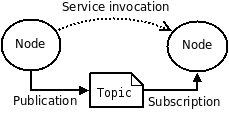
\includegraphics[width=0.5\textwidth]{drive/ROS_concepts.png}
	\caption{ROS Nachrichtenkonzept}
	\label{fig:ROS_concepts}
\end{figure}

Falls diese Daten folgend von einer anderen Node benötigt werden, kann diese das Topic einfach abhören und bekommt ausschließlich die gewünschten Daten übermittelt. Mit Hilfe des Nachrichtensystems lässt sich der Ablauf und die Synchronisation von einzelnen Funktionen des Roboters übersichtlich und einfach gestalten. Darüber hinaus bietet ROS praktische Tools zur Visualisierung von Messdaten, wie z.B. Laserscans.

\subsubsection*{Was will ROS?}
\begin{itemize}
 \item ROS will unterstützen, Code für Forschung und Entwicklung wiederzuverwenden
 \item loser Verbund von individuellen Programmteilen (Nodes)
 \item einzelne Programmteile können einfach geteilt und verbreitet werden (Packages und Stacks)
 \item ROS stellt Repositories zu Verfügung, um dort Code zu teilen \cite{ROS:2014:Online}
(http://www.ros.org/browse)
\end{itemize}
\subsubsection*{Was kann ROS?}
Die Hauptbestandteile und Hauptaufgaben von ROS sind Hardwareabstraktion; Gerätetreiber; Implementierung 
von viel genutzten Funktionalitäten; Inter-Prozess-Kommunikation; Paket-Management
\subsubsection*{Aufgaben des ROS}
\begin{itemize}
 \item Interprozesskommunikation (IPC)
 \begin{itemize}
\item Problematik der Kommunikation zwischen verschiedenen Systemen des Roboters
\item Sicherheitseinstellung bei der Übertragung
\item Anforderung an die Geschwindigkeit / Schnelligkeit der Kommunikation
\item Koordination von Nachrichten durch zentralen Master
\end{itemize}
\item Paketverwaltung – Packages
\begin{itemize}
 \item ROS ist durch Softwarepakete (sogn. Packages) aufgebaut
 \item Ein Package beinhaltet Laufzeitprozesse (Nodes); ROS abhängige Bibliotheken;
Datensätze; Konfigurationsdateien;3rd Party Software
 \item Packages sind dazu, da um Code wiederverwendbar zu machen
\end{itemize}
\item Paketverwaltung – Stacks
\begin{itemize}
\item Sammlung von Paketen (Packages)
\item Der Sinn ist, dass Stacks die Verteilung und Verwendbarkeit von Code
vereinfachen
\item Meist viele Packages ähnlicher Aufgaben in einem Stack verpackt
\end{itemize}
\item Message (msg)
\begin{itemize}
 \item  Messages werden verwendet um unter ROS Nachrichten zwischen Knoten und
Topics auszutuaschen
\item Dafür verwendet ROS eine einfache Beschreibung der Datentypen in Textdateien
\item Durch diese Beschreibung kann für unterschiedliche Sprachen Code autogeneriert
werden
\item Diese sind in .msg-Dateien im msg- Unterverzeichnis eines ROS-Pakets abgelegt
\item Eigene Message-Typen sind mit Paket Ressource-Namen bezeichnet
\item Standard Messages sind mit std\_msg/msg/String.msg bezeichnet
\end{itemize}
\item Service
\begin{itemize}
 \item ROS verwendet eine eigene vereinfachte Service Description Language ("srv") für die
Beschreibung von ROS Service-Typen
\item Setzt direkt auf die ROS msg-Format auf
\item Ermöglicht die Anfrage / Antwort-Kommunikation zwischen den Knoten
\item Service-Beschreibungen sind in .srv-Dateien im srv- Unterverzeichnis eines Pakets
gespeichert
\item Service-Beschreibungen werden für die Verwendung mit dem Paket Ressource-
Namen bezeichnet
\item Z. B.: wird die Datei robot\_srvs/srv/SetJointCmd.srv als Service
robot\_srvs/SetJointCmd bezeichnet
\end{itemize}
\item Notes
\begin{itemize}
 \item Der Nachrichtenaustausch findet bei Nodes durch 3 Möglichkeiten statt: Parameter
Server;Topics; Services
\item Nodes werden wie in einem Graph angeordnet
\item In einem System laufen viele Nodes Parallel
\item Diese werden zu Beginn gestartet
\item Beispiele sind Nodes für: Laserscanner; Kinect; Pfadplanung
\end{itemize}
\item Topica
\begin{itemize}
 \item Topics verhalten sich wie ein virtuelles BUS-System Nodes können von Topics lesen
(subscribe)
\item Nodes können an Topics senden (publish)
\item Es gibt keine Begrenzung wie viele Nodes publsih oder subscribe auf ein Topic
machen
\end{itemize}
\end{itemize}
\subsubsection*{ROS-Datensystem}
ROS-Ressourcen sind in rangmäßiger Gliederung eingeordnet. Zwei Konzepte sind zu
verstehen:
\begin{itemize}
\item \textbf{Le package}: Es handelt sich hier um die Zentraleinheit der Softwareorganisation von
ROS. Ein Package ist ein Verzeichnis der die Knoten beinhaltet (wir werden hier
unten erklären, was ein Knoten ist) sowie die externen Librairies, Daten und XML
Konfigurationsdateien die manifest.xml genannt wird.
\item \textbf{Stack}: Stack bezeichnet eine Sammlung von Packagen. Sie ermöglicht mehrere
Funktionen wie Navigation, Lokalisierung und viele mehr. Ein Stack beinhaltet
mehrere Verzeichnisse sowie eine Konfigurationsdatei die stack.xml genannt wird.
\begin{itemize}
\item Vorhandene wichtige Stacks
\begin{itemize}
\item TF – Koordinatentransformation
\item Navigationstack
\item URDF - Modelle
\end{itemize}
\begin{itemize}
\item Beispiel Navigationstack
\begin{itemize}
\item Wertet Sensordaten aus z.B.: Laserdaten
\item Baut daraus mit gmapping (ebenfalls ein ROS-Stack) eine Begehbarkeitskarte
\item Warum? Zur Kollisionsvermeidung
\item Bei erfolgreicher Erstellung einer Map kann dann ein Ziel übergeben werde (Pfadplanung durch Navigationstack,
Kollisionsvermeidung, Reaktion auf sich ändernde Umgebung, Aufbau einer globalen Karte)
\end{itemize}
\end{itemize}
\end{itemize}
\end{itemize}
\subsubsection*{Vorteile und Nachteile des ROS}
\paragraph*{Vorteile}
\begin{itemize}
 \item Nachrichten-basierte Software Architektur
\begin{itemize}
\item Verschiedene Komponenten sind unabhängig voneinander mit dem System verbunden
\item Unterschiedliche Komponenten können miteinander verbunden werden, ohne jedes Mal das Programm neu zu Kompilieren
\item Netzwerkfähigkeit
\item Einfaches Debugging und Simulieren
\end{itemize}
\item Absturz eines Nodes führt nicht zum Absturz des ganzen
Systems
\item Für ROS lässt sich in mehreren Sprachen programmieren
\item ROS hat eine große Community, die viele Daten und Programme zu Verfügung
stellen
\end{itemize}
\paragraph*{Nachteile}
\begin{itemize}
 \item Durch Nachrichten-basierte Systemarchitektur Bottleneck bei großer Datenmenge
\item Steuerung des Systems über Kommandozeile
\end{itemize}

\subsubsection{Epos Control}

\subsubsection{SOPAS Engineeringtool}

Bei SOPAS ET handelt es sich um ein Entwicklungsprogramm von Sick. Dieses wird zur Ansteuerung und Konfiguration der Laserscanner und Hallsensosren verwendet.

\begin{itemize}
\item \textbf{ Erster Start }

Beim ausführen von SOPAS wird ein neues Projekt erstellt, in dem man die gewünschte Hardware selektiert und einbindet. Die Wahl der Hardware erfolgt hierbei über den Netzwerkscanassistenten oder manuell über den Gerätekatalog. Sobald die Kommunikation mit der Hardware aktiv ist, kann diese angesteuert werden. Änderungen der Konfiguration der Hardware sind im Projektbaum möglich oder sogar notwendig ( siehe Kapitel 7.7 Herausforderungen).
\end{itemize}
